%导言区
\documentclass{ctexart}%ctexbook, ctexrep
%\usepackage{ctex}
%导言区: \usepackage{graphicx}
%语法:\includegraphics[< 选项>]{< 文件名》}
%格式: EPS, PDF, PNG,JPEG, BMP
\usepackage{graphicx}
\graphicspath{{figures/},{pic/}} %图片在当前目录下的figures目录,大括号实现分组。
%正文区(文稿区)
\begin{document}
	\LaTeX{ }中的插图:
	
	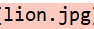
\includegraphics{lion}
	
	\includegraphics{mountain}
	
	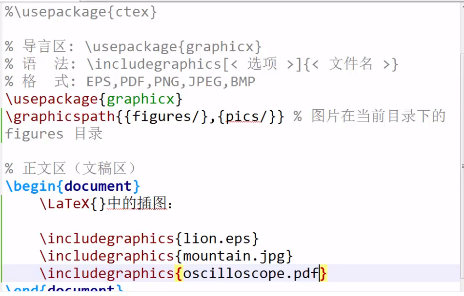
\includegraphics{oscilloscope}
	
	%缩放因子(倍数)
	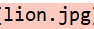
\includegraphics[scale=0.3]{lion}
	\includegraphics[scale=0.03]{mountain}
	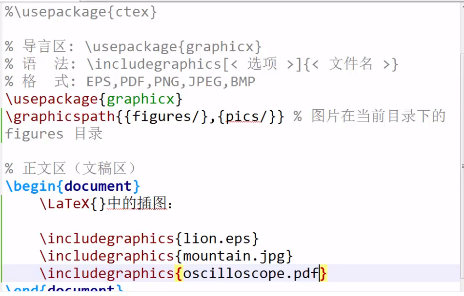
\includegraphics[scale=0.3]{oscilloscope}
	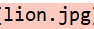
\includegraphics[height=2cm]{lion}
	\includegraphics[height=2cm]{mountain}
	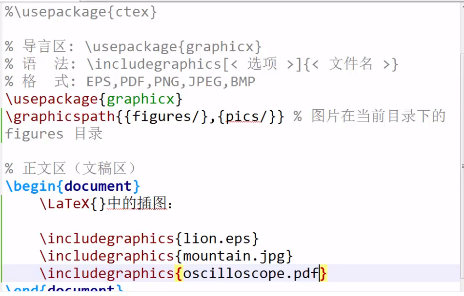
\includegraphics[height=2cm]{oscilloscope}
	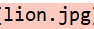
\includegraphics[width=2cm]{lion}
	\includegraphics[width=2cm]{mountain}
	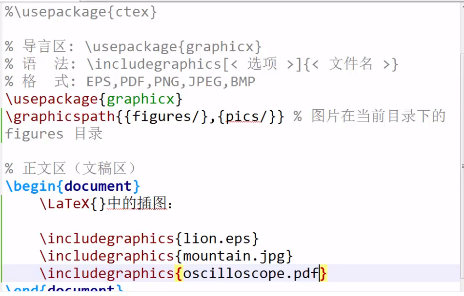
\includegraphics[width=2cm]{oscilloscope}
	%版型文本高度0.1倍的图像高度(高度一致)
	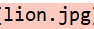
\includegraphics[height=0.1\textheight]{lion}
	\includegraphics[height=0.1\textheight]{mountain}
	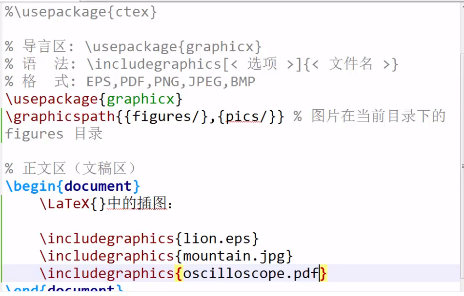
\includegraphics[height=0.1\textheight]{oscilloscope}
	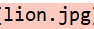
\includegraphics[width=0.2\textwidth]{lion}
	\includegraphics[width=0.2\textwidth]{mountain}
	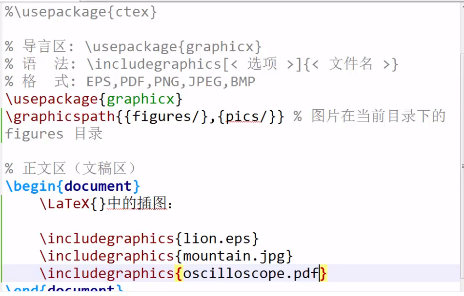
\includegraphics[width=0.2\textwidth]{oscilloscope}
	%不同参数之间逗号进行分割
	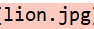
\includegraphics[angle=-45,
	width=0.2\textwidth]{lion}
	\includegraphics[width=0.2\textwidth]{mountain}
	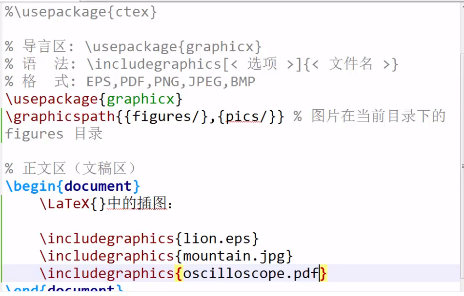
\includegraphics [angle=45,
	width=0.2\textwidth]{oscilloscope}
\end{document}